
La técnica de PCR es una técnica de biología molecular desarrollada en 1983 por Kary Mullis.

Su objetivo es, a partir de una mínima cantidad de ADN, obtener un gran número de copias de un fragmento de ADN particular; en teoría basta partir de una sola copia de ese fragmento original, o molde, para crea una gran cantidad de copias del mismo.

\section{Desarrollo de la PCR}





\section{Procedimiento común de una PCR clásica}

La PCR funciona subiendo y bajando la temperatura de las muestras de ADN, esto para que ocurran las diferentes reacciones que permiten la generación de copias de ADN. Esto se compone de \textbf{3 pasos} que se repiten una y otra vez, y es lo que se conoce como \textbf{ciclo}.

%\begin{figure}[H]
%    \centering
%    \resizebox{\linewidth}{!}{\input{images/fig:ciclos_de_la_pcr}}
%    \rule{\linewidth}{0.5pt}
%    \caption{Ciclo básico de una PCR}
%    \label{fig:ciclos_de_la_pcr}
%\end{figure}

\begin{enumerate}
    \item \textbf{Desnaturalización:}En este primer paso, se aumenta la temperatura de la muestra de ADN, esto para hacer que la doble hélice se separe y que las hebras estén "disponibles" para que la polimerasa pueda realizar  su trabajo (elongar). La temperatura a la que se lleva suele estar \textbf{entre 93 y 98°C}, usualmente usandose el punto medio, 95°C. Esta temperatura se mantiene durante, aproximadamente \textbf{30 segundos}. 
    \item \textbf{Alineación:} Una vez separadas las cadenas de ADN, los primers se unen al sector para el que fueron diseñados, esto para que la polimerasa pueda tener un sector desde el cual iniciar. Para este paso la temperatura se reduce hasta \textbf{45-60°C}, y se mantiene así aproximadamente \textbf{30 segundos}.
    \item \textbf{Elongación:} Una vez separadas las hebras de ADN y que los primers se hubieran unido a este ADN, la polimerasa puede elongar los sectores de interés. Aquí se vuelve a aumentar la temperatura hasta \textbf{65-72°C} durante \textbf{1 minuto}.
\end{enumerate}

La PCR clásica tiene la desventaja de necesitar un proceso posterior (electroforesis en gel) para poder cuantificar la cantidad de ADN obtenido.

Posterior a una PCR clásica, se realiza una electroforesis en gel. Para realizar esta electroforesis se usa un \textbf{buffer TAE} (Tris-Acetato-EDTA). A la muestra se añade un \textbf{buffer de carga} (\textit{loading buffer}) y un \textbf{colorante de ADN}. RedGel es el más usado, pero aún se llega a utilizar bromuro de etidio, pero se ha reducido su uso por sus efectos tóxicos para la salud. Usualmente los buffer de carga ya vienen cargados con colorante RedGel.

\marginpar{\begin{minipage}{\marginparwidth}
    \begin{figure}[H]
        \centering
        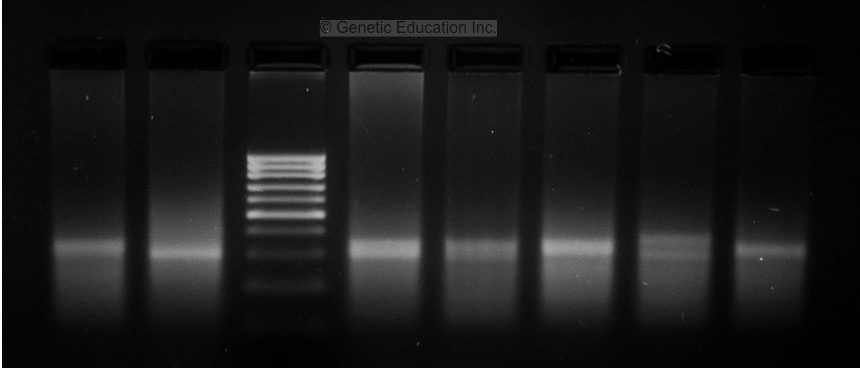
\includegraphics[width=\linewidth]{images/fig:electroforesis_en_gel_de_pcr}
        \rule{\linewidth}{0.5pt}
        \caption{Ejemplo de una electroforesis en gel}
        \label{fig:electroforesis_en_gel_de_pcr}
    \end{figure}
\end{minipage}}

El gel se prepara haciendo uso de \textbf{agarosa}, cuya concentración suele estar entre 1 y 2\%. La concentración exacta dependerá del tamaño del ADN que se busque generar. Con ADN "pequeño", se prepara un gel de alta concentración (2\%), mientras que cuando se busca ADN más "grande" se preparaun gel menos concentrad (1\%).














\section{Variantes de la PCR}

Existen diferentes formas de realizar la PCR, sin embargo, el proceso de la PCR descrito anteriormente suele variar poco entre estos métodos. Los tipos de PCR principales son:

\begin{itemize}
    \item Tiempo real (qPCR)
    \item Retrotranscriptasa (RT-PCR)
    \item Combinación Retrotranscriptasa-Tiempo Real (RT-qPCR)
    \item Digital
\end{itemize}

\subsection{Tiempo real (qPCR)}

Este también sigue los pasos anteriormente descritos, pero hace uso de termocicladores que miden la cantidad de ADN generado al mismo tiempo que llevan el proceso de PCR.
Esto se logra agregando sustancias que pueden ser medidas mediante espectrofotometría, y después de cada ciclo el termociclador toma una medición de estas sustancias mediante el uso de \textbf{luz UV}.

\marginpar{\begin{minipage}{\marginparwidth}
    \begin{figure}[H]
        \centering
        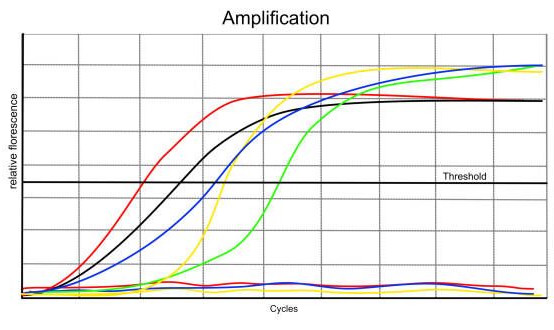
\includegraphics[width=\linewidth]{images/fig:grafica_de_qpcr}
        \rule{\linewidth}{0.5pt}
        \caption{Ejemplo de una gráfica resultante de una qPCR}
        \label{fig:grafica_de_qpcr}
    \end{figure}
\end{minipage}}

Este proceso necesita de material de referencia y da como resultado una gráfica que usualmente se ve como una \textbf{curva sigmoide}, cuyo eje x mide los ciclos que pasan y el eje y es la absorbancia.

\begin{figure}[H]
    \centering
    \resizebox{\linewidth}{!}{\input{images/fig:ciclo_de_qpcr}}
    \rule{\linewidth}{0.5pt}
    \caption{Ciclo de una qPCR}
    \label{fig:ciclo_de_qpcr}
\end{figure}

En el caso de una qPCR, el software del termociclador ya realiza una cuantificación de ADN, esto a través de la adición de colorantes antes de la realización de la PCR.

\subsubsection{SYBR Green}

Este es un colorante que se une a las cadenas dobles de ADN y que tiene cuerta fluorescencia, esto para hacerlas cuantificables por el equipo.

Este método \textbf{no es tan exacto}, esto porque que este colorante se une a todas las cadenas dobles de la muestra, no diferencia entre las originales y las generadas por la polimerasa. Para resolver esta incertidumbre se realiza una \textbf{curva de Melting}.

\marginpar{\begin{minipage}{\marginparwidth}
    \begin{figure}[H]
        \centering
        \resizebox{\linewidth}{!}{\definecolor{primercolor}{RGB}{250,165,60}
\definecolor{dntpscolor}{RGB}{135,195,195}

\begin{tikzpicture}[
    titulo/.style={midway, above=0pt, font=\sffamily\bfseries\Large},
    cadena/.style={line width=3pt},
    primer/.style={line width=2pt, color=primercolor},
    dntps/.style={draw, fill=dntpscolor},
    active dntp/.style={draw, fill=dntpscolor, decorate, decoration=bumps},
    texto/.style={midway, font=\sffamily\footnotesize}
]

% Desnaturalización
\draw[line width=0.5pt] (3,0) -- (7,0) node[titulo] {Desnaturalización};

\draw[primer, -Stealth] (1,-1) --++ (2,0) node[texto, above=0pt, pos=0.45] {Primer};
\draw[cadena] (0,-3) --++ (6,0);
\draw[cadena] (4,-6) --++ (6,0);
\draw[primer, Stealth-] (7,-8) --++ (2,0) node[texto, below=0pt, pos=0.55] {Primer};

\draw[dntps] (4.75,-1.75) circle (0.3cm);
\draw[dntps] (6.6,-1.12) circle (0.3cm);
\draw[dntps] (8,-2.25) circle (0.3cm);
\draw[dntps] (9.25,-1.25) circle (0.3cm);
\draw[dntps] (9,-4) circle (0.3cm);
\draw[dntps] (0.85,-4.5) circle (0.3cm);
\draw[dntps] (2.15,-6) circle (0.3cm);
\draw[dntps] (0.85,-7.25) circle (0.3cm);
\draw[dntps] (3.75,-7.75) circle (0.3cm);
\draw[dntps] (5.5,-7) circle (0.3cm);

% Alineación
\draw[line width=0.5pt] (3,-10) -- (7,-10) node[titulo] {Alineación};

\draw[primer, -Stealth] (1,-12) --++ (2,0) node[texto, above=0pt, pos=0.45] {Primer};
\draw[cadena] (0.25,-13) --++ (6,0);
\draw[cadena] (4,-16) --++ (6,0);
\draw[primer, Stealth-] (7,-17) --++ (2,0) node[texto, below=0pt, pos=0.55] {Primer};

\draw[active dntp] (1.5,-12.5) circle (0.2cm);
\draw[active dntp] (2.2,-12.5) circle (0.2cm);
\draw[dntps] (6,-11) circle (0.3cm);
\draw[dntps] (8.25,-11.75) circle (0.3cm);
\draw[dntps] (9.75,-13.25) circle (0.3cm);
\draw[dntps] (1.1,-16) circle (0.3cm);
\draw[dntps] (2.5,-16.75) circle (0.3cm);
\draw[dntps] (5,-17.25) circle (0.3cm);
\draw[active dntp] (7.8,-16.5) circle (0.2cm);
\draw[active dntp] (8.5,-16.5) circle (0.2cm);

% Elongación
\draw[line width=0.5pt] (3,-20) -- (7,-20) node[titulo] {Elongación};

\draw[cadena, -Stealth] (0,-23) --++ (7,0);
\draw[cadena] (0,-22) --++ (5,0);
\draw[cadena] (4,-26) --++ (6,0);
\draw[cadena, Stealth-] (3,-27) --++ (7,0);

\draw[active dntp] (0.5,-22.5) circle (0.2cm);
\draw[active dntp] (1.5,-22.5) circle (0.2cm);
\draw[active dntp] (2.5,-22.5) circle (0.2cm);
\draw[active dntp] (3.5,-22.5) circle (0.2cm);
\draw[active dntp] (4.5,-22.5) circle (0.2cm);
\draw[active dntp] (5.5,-22.5) circle (0.2cm);
\draw[dntps] (9.5,-23.7) circle (0.3cm);
\draw[dntps] (1.36,-26.44) circle (0.3cm);
\draw[active dntp] (4.5,-26.5) circle (0.2cm);
\draw[active dntp] (5.5,-26.5) circle (0.2cm);
\draw[active dntp] (6.5,-26.5) circle (0.2cm);
\draw[active dntp] (7.5,-26.5) circle (0.2cm);
\draw[active dntp] (8.5,-26.5) circle (0.2cm);
\draw[active dntp] (9.5,-26.5) circle (0.2cm);
\end{tikzpicture}}
        \rule{\linewidth}{0.5pt}
        \caption[Funcionamiento del colorante SYBR-Green]{Los círculos representan el SYBR-Green que \textbf{no emite luz}, mientras que las ``estrellas'' representan el SYBR-Green que \textbf{ya emite luz}.}
        \label{fig:sybr_green}
    \end{figure}
\end{minipage}}

\subsubsection{Sonda Taq-Man}

Las sondas Taq-Man son moléculas que se componen de una cadena de nucleótidos que contiene un \textbf{fluoroforo (reportero)} en el \textbf{extremo 5'} y un \textbf{desactivador de fluorescencia (quencher)} en el \textbf{extremo 3'}.
Cuando se añaden las sondas a la muestra y las ADN se abren, las sondas se unen a zonas determinadas del ADN, pero por como están conformadas aún no pueden emitir luz que el termociclador pueda medir. Cuando inicia la PCR, la polimerasa avanza por la cadena de ADN y al llegar a la sonda Taq-Man la retira. Una vez liberada, los componentes de esta se separan y el reportero puede, ahora sí, emitir luz que puede ser medida por el termociclador.

Estas sondas, a comparación del SYBR Green, es \textbf{más específico}, pues hace que solo se midan las cadenas de ADN generadas, y no las originales de la muestra.

\marginpar{\begin{minipage}{\marginparwidth}
    \begin{figure}[H]
        \centering
        \resizebox{\linewidth}{!}{\definecolor{primercolor}{RGB}{250,165,60}
\definecolor{reportercolor}{RGB}{135,185,185}
\definecolor{reporteractcolor}{RGB}{70,210,135}
\definecolor{quenchercolor}{RGB}{245,155,140}
\definecolor{taqmancolor}{RGB}{120,185,225}
\definecolor{Gris}{RGB}{165,165,165}

\begin{tikzpicture}[
    titulo/.style={anchor=west, font=\sffamily\bfseries\Large},
    separador/.style={line width=1pt, color=Gris},
    cadena/.style={line width=1.5pt},
    cadena nueva/.style={line width=1.5pt, color=Gris},
    primer/.style={line width=1.5pt, color=primercolor},
    texto/.style={font=\sffamily\scriptsize},
    taqman/.style={circle, texto},
    r/.style={fill=reportercolor},
    activo/.style={fill=reporteractcolor, decorate, decoration=bumps},
    q/.style={fill=quenchercolor}
]

% Alineación
\def\DesnatY{0}
\node[titulo] (desnaturalizacion) at (0,\DesnatY) {Alineación de primers};
\draw[primer, -Stealth] (0,\DesnatY-2) --++ (2,0) node[texto, midway, above=0pt, pos=0.45] {Primer};
\draw[cadena] (0,\DesnatY-2.5) --++ (10,0);
\draw[cadena] (0,\DesnatY-3.5) --++ (10,0);
\draw[primer, Stealth-] (8,\DesnatY-4) --++ (2,0) node[texto, midway, below=0pt, pos=0.55] {Primer};
\node[taqman, r] (r1) at (4,\DesnatY-1.75) {R};
\node[taqman, q] (q1) at (6,\DesnatY-1.75) {Q};
\draw[line width=2pt, color=taqmancolor] (r1.south) --++ (0,-0.25) --++ (2,0) node[midway, above=0pt, black, texto] {Sonda} -- (q1.south);

% Elongación
\def\AlinY{-6}
\node[titulo] (alineacion) at (0,\AlinY) {Elongación};
\draw[primer] (0,\AlinY-2) --++ (2,0);
\draw[cadena nueva, -Stealth] (2,\AlinY-2) --++ (1.75,0);
\draw[cadena] (0,\AlinY-2.5) --++ (10,0);
\draw[cadena] (0,\AlinY-3.5) --++ (10,0);
\draw[cadena nueva, Stealth-] (6.25,\AlinY-4) --++ (1.75,0);
\draw[primer] (8,\AlinY-4) --++ (2,0);
\node[taqman, r] (r2) at (3.75,\AlinY-1.5) {R};
\node[taqman, q] (q2) at (6,\AlinY-1.75) {Q};
\draw[line width=2pt, color=taqmancolor] (q2.south) --++ (0,-0.25) --++ (-2,0) -- (r2.south);

% Escición
\def\EscY{-12}
\node[titulo] (escicion) at (0,\EscY) {Escición de la sonda};
\draw[primer] (0,\EscY-2) --++ (2,0);
\draw[cadena nueva, -Stealth] (2,\EscY-2) --++ (2.5,0);
\draw[cadena] (0,\EscY-2.5) --++ (10,0);
\draw[cadena] (0,\EscY-3.5) --++ (10,0);
\draw[cadena nueva, Stealth-] (5.5,\EscY-4) --++ (2.5,0);
\draw[primer] (8,\EscY-4) --++ (2,0);
\node[taqman, r, activo] (r3) at (3.5,\EscY-1.25) {R};
\node[taqman, q] (q3) at (6,\EscY-1.75) {Q};
\draw[line width=2pt, color=taqmancolor] (q3.south) --++ (0,-0.25) --++ (-1,0);

% Detección
\def\ElonY{-18}
\node[titulo] (elongacion) at (0,\ElonY) {Detección de la señal};
\draw[primer] (0,\ElonY-2) --++ (2,0);
\draw[cadena nueva, -Stealth] (2,\ElonY-2) --++ (8,0);
\draw[cadena] (0,\ElonY-2.5) --++ (10,0);
\draw[cadena] (0,\ElonY-3.5) --++ (10,0);
\draw[cadena nueva, Stealth-] (0,\ElonY-4) --++ (8,0);
\draw[primer] (8,\ElonY-4) --++ (2,0);
\node[taqman, r, activo] (r4) at (4,\ElonY-1) {R};
\node[taqman, q] (q4) at (8,\ElonY-1) {Q};
\draw[line width=2pt, color=taqmancolor] (q4.south) --++ (0,-0.25) --++ (-1,0);
\end{tikzpicture}}
        \rule{\linewidth}{0.5pt}
        \caption{Funcionamiento de las sondas Taq-Man}
        \label{fig:sondas_taqman}
    \end{figure}
\end{minipage}}





\subsection{Retrotranscriptasa-PCR (RT-PCR)}

Este, más que un método de PCR, es un paso que se realiza previo a la PCR. Cuando se cuenta con muestras de ARN, es necesario convertirlas a ADN, por lo que se utiliza la \textbf{enzima RT} (retro-transcriptasa) para realizar tal conversión. Una vez realizado esto, se puede proseguir con la técnica de PCR que se desee. La polimerasa usada en la PCR trabaja con ADN, por lo que de querer analizar muestras de ARN (por ejemplo, muestras de virus) se necesita transformar el ARN en ADN. Para esto se usa una enzima llamada retrotranscriptasa o transcriptasa inversa, también abreviada como enzima RT. Esta enzima convierte ARN's en ADN complementario (ADNc), y se usa previo a la PCR añadiendo las enzimas RT y temperatura, usualmente de entre 45-50°C durante 30 minutos, aunque las temperaturas y tiempos exactos van a variar dependiendo el contexto.

\marginpar{ {\rule{\marginparwidth}{2pt}} \footnotesize
Una RT ampliamente usada es la MMLV-RT (Moloney Murine Leukemia Virus - Retro-Transcriptase), aislada del virus de la leucemia murina de Moloney.
}

\begin{figure}[H]
    \centering
    \resizebox{\linewidth}{!}{\input{images/fig:ciclo_de_rt_pcr}}
    \rule{\linewidth}{0.5pt}
    \caption{Metodología de una RT-PCR}
    \label{fig:ciclo_de_rt_pcr}
\end{figure}



\subsection{RT-qPCR}

Se abrevia así cuando se realizan el proceso de RT-PCR seguido de una qPCR.

\begin{figure}[H]
    \centering
    \resizebox{\linewidth}{!}{\begin{tikzpicture}[
    paso/.style={draw, rounded corners=2pt, align=center, text width=10em, inner sep=5pt, font=\sffamily\bfseries, anchor=west},
    especificacion/.style={draw, densely dashed, rounded corners=2pt, align=center, text width=5em, inner sep=5pt, font=\sffamily\small},
    flecha/.style={-Stealth, line width=1pt}
]

\node[paso] (desnaturalizacion) at (0,0) {1. Desnaturalización};
\node[especificacion] (desnaturalizacion esp) at ([yshift=-1.5cm]desnaturalizacion) {93-98\celsius\\30 seg.};
\draw[dotted, line width=0.5pt] (desnaturalizacion) -- (desnaturalizacion esp);

\node[paso] (alineacion) at ([xshift=2cm]desnaturalizacion.east) {2. Alineación};
\node[especificacion] (alineacion esp) at ([yshift=-1.5cm]alineacion) {45-60\celsius\\30 seg.};
\draw[dotted, line width=0.5pt] (alineacion) -- (alineacion esp);

\node[paso] (elongacion) at ([xshift=2cm]alineacion.east) {3. Elongación};
\node[especificacion] (elongacion esp) at ([yshift=-1.5cm]elongacion) {65-72\celsius\\1 min.};
\draw[dotted, line width=0.5pt] (elongacion) -- (elongacion esp);

\draw[flecha] (desnaturalizacion.east) -- (alineacion.west);
\draw[flecha] (alineacion.east) -- (elongacion.west);
\draw[flecha] (elongacion.north) to[out=135,in=0] ([yshift=1.25cm]alineacion.north) to[out=180,in=45] (desnaturalizacion.north); 

\node[especificacion] (colorante) at ([xshift=-2cm]desnaturalizacion.west) {0.2. Agregar colorante};
\node[especificacion] (rt) at ([xshift=-2cm]colorante.west) {0.1. Convertir ADN a ARN con RT};

\draw[dashed, line width=0.5pt, -Stealth] (rt) -- (colorante) -- (desnaturalizacion);
\end{tikzpicture}}
    \rule{\linewidth}{0.5pt}
    \caption{Metodología de una RT-qPCR}
    \label{fig:ciclo_de_rt_qpcr}
\end{figure}

\subsection{Digital}
En este método, el proceso está casi completamente automatizado mendiante el uso de máquinas especializadas.














